%%%%%%%%%%%%%%%%%%%%%%%%%%%%%%%%%%
% EL/EEE D1 Report Template
% University of Southampton
%
% author : Rhys Thomas (rt8g15)
%
% edited : 2016-11-14
%%%%%%%%%%%%%%%%%%%%%%%%%%%%%%%%%%

\documentclass[a4paper,11pt]{article}

%%%%%%%%%%%%%%%%%%%%%%%%%%%%%%%%%%
% PACKAGES
%%%%%%%%%%%%%%%%%%%%%%%%%%%%%%%%%%
\usepackage[margin=1in]{geometry}
\usepackage{wrapfig,lipsum,booktabs}

\usepackage{graphicx}
\usepackage{csvsimple}
\usepackage{caption}
\usepackage{wrapfig}
\usepackage{siunitx}
\usepackage{fixltx2e}
\usepackage{colortbl}
%\usepackage{float}
\usepackage{floatrow}
\usepackage{amsmath}
\usepackage[T1]{fontenc}
\usepackage{bigfoot} % to allow verbatim in footnote
\usepackage[numbered,framed]{matlab-prettifier}
\usepackage{subfig}
\usepackage{siunitx}

\usepackage{listings}
\usepackage{color} %red, green, blue, yellow, cyan, magenta, black, white
\definecolor{mygreen}{RGB}{28,172,0} % color values Red, Green, Blue
\definecolor{mylilas}{RGB}{170,55,241}
\usepackage{graphicx}

\usepackage[titletoc,toc,title]{appendix}
\renewcommand{\baselinestretch}{1.2} % line spacing


\lstset{
	style              = Matlab-editor,
	basicstyle         = \mlttfamily,
	escapechar         = ",
	mlshowsectionrules = true,
}


%%%%%%%%%%%%%%%%%%%%%%%%%%%%%%%%%%
% DOCUMENT BEGIN
%%%%%%%%%%%%%%%%%%%%%%%%%%%%%%%%%%
\begin{document}
 
\setlength{\parindent}{0cm}
\begin{center}

{\Large{\textbf{ELEC2205 Electronic Design:\\ D3 -- Analogue Circuit Design Exercise}}} \\ [\baselineskip]	
Jemma Watson \\
jw14g15 \\
Tutor: Dr Tracy Melvin \\
\end{center}

\section{Derivations}

\subsection{First stage: Common Emitter Circuit}
The first circuit can be identified as a common emitter stage with partially by-passed emitter resistance. 

\begin{figure}[H]
	\centering
	\subfloat{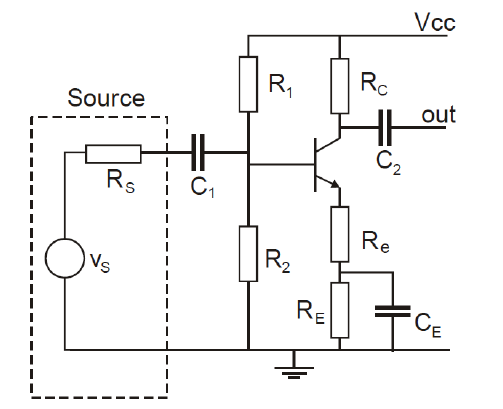
\includegraphics[width=5cm]{figures/emitter}}
	\label{fig:emitter}
	\hfill
\end{figure}

\subsubsection{Mid-band Gain}
\begin{figure}[H]
	\centering
	\subfloat{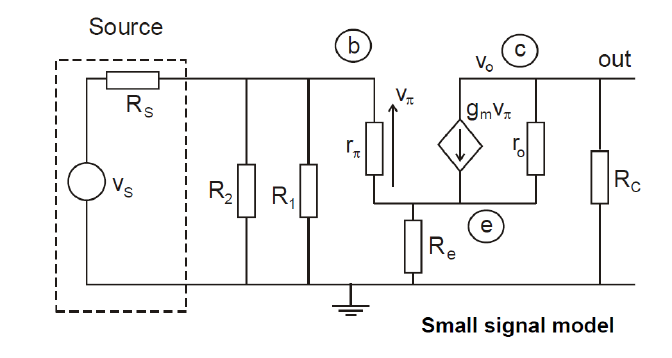
\includegraphics[width=10cm]{figures/ss_emitter}}
	\caption{Small signal model of common emitter}
	\label{fig:ss_emitter}
	\hfill
\end{figure}


By performing nodal analysis on Figure \ref{fig:ss_emitter}, the following equations can be obtained.

\begin{subequations}
	\begin{align}
		\textrm{Base: } &\frac{v_b - v_s}{R_s} + \frac{v_b}{R_1} + \frac{v_b}{R_2} + \frac{v_b - v_e}{r_\pi} &= 0 \nonumber \\ 
		&\frac{v_b - v_s}{R_s} + v_b \left(\frac{1}{R_1} + \frac{1}{R_2} \right) + \frac{v_b - v_e}{r_\pi} &= 0 \label{eq:base} \\
		\textrm{Emitter: }	&\frac{v_e - v_b}{r_\pi} + g_m v_\pi + \frac{v_e}{R_e} &= 0\nonumber \\ 
		&\frac{v_e - v_b}{r_\pi} - g_m (v_b-v_e) + \frac{v_e}{R_e} &= 0 \label{eq:emitter} \\
		\textrm{Collector: }	&\frac{v_c}{R_c} + g_m (v_b-v_e) &= 0\label{eq:collector}
	\end{align}
\end{subequations}

Rearranging equation \ref{eq:emitter}


\begin{align*}
		v_e [\frac{1}{r_\pi} + \frac{1}{R_e}+g_m] &= \frac{v_b}{r_\pi} + g_m v_b \\
		v_e [R_e (1+g_m r_\pi) +r_\pi] &= v_b R_e (1+g_m r_\pi)
\end{align*}

Using the fact that $g_m r_\pi=\beta$
\begin{align}
	v_e = v_b R_e (\frac{1 + \beta}{R_e (1 + \beta) + r_\pi}) \label{eq:ve}
\end{align}

Modifying equation \ref{eq:collector} as such
\begin{align*}
\frac{v_c}{R_c} + g_m (v_b-v_e) &= 0 \\ 
\frac{v_c}{R_c} + g_m v_b &= g_m v_e \\
v_e &= \frac{v_c}{g_m R_c} + v_b
\end{align*}

gives a value of $v_e$ that can be substituted back into equation \ref{eq:ve}
\begin{align*}
v_b R_e (\frac{1 + \beta}{R_e (1 + \beta) + r_\pi}) &= \frac{v_c}{g_m R_c} + v_b \\
v_b R_e (1 + \beta) &= \frac{v_c (R_e (1 + \beta) + r_\pi)}{g_m R_c} + v_b (R_e (1 + \beta) + r_\pi) \\
-v_b r_\pi &= \frac{v_c (R_e (1 + \beta) + r_\pi)}{g_m R_c} \\
\frac{v_c}{v_b} &= - \frac{r_\pi g_m R_c}{R_e (1 + \beta) + r_\pi} \\
\frac{v_c}{v_b} &= - \frac{\beta R_c}{R_e (1 + \beta) + r_\pi}
\end{align*}

This may be approximated as 
\begin{align}
A &= - \frac{\beta R_c}{R_e (1 + \beta) + r_\pi} \approx -\frac{R_c}{R_e}
\end{align}

\subsubsection{Input Impedance}
The impedance into the base terminal of the common emitter circuit is given by 

\begin{align*}
R_b &= \frac{v_b}{i_b} \\
\textrm{Where } i_b &= \frac{v_b - v_e}{r_\pi}
\end{align*}

Therefore
\begin{align}
R_b &= \frac{v_b r_\pi}{v_b - v_e} \nonumber \\
	&= \frac{r_\pi}{1 - \frac{v_e}{v_b}} \label{eq:rb}
\end{align}

From equation \ref{eq:ve}
\begin{align}
	\frac{v_e}{v_b} = R_e (\frac{1 + \beta}{R_e (1 + \beta) + r_\pi}) \label{eq:ve_rearranged}
\end{align}

Substituting equation \ref{eq:ve_rearranged} into \ref{eq:rb} and rearranging gives gives
\begin{align*}
	R_b = r_\pi + R_e (\beta + 1)
\end{align*}

Therefore input impedance is the parallel combination of $R_1$, $R_2$ and $R_b = r_\pi + R_e (\beta + 1)$

\begin{align}
	R_i = ( \frac{1}{R_1} + \frac{1}{R_2} + \frac{1}{r_\pi + R_e (\beta + 1)} )^{-1} \label{eq:input_inpedance_emitter}
\end{align}

\subsubsection{Output Impedance}
By examining \ref{fig:ss_emitter} it can be seen that the output impedance will be
\begin{align}
R_o = R_c \label{eq:output_inpedance_emitter}
\end{align}


\subsection{Common Collector Circuit}
The second stage of the circuit consists of a straight forward common collector circuit as shown in figure \ref{fig:collector}.

\begin{figure}[H]
	\centering
	\subfloat{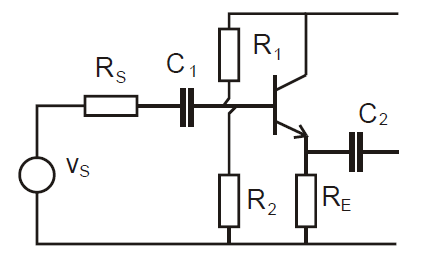
\includegraphics[width=5cm]{figures/collector}}
	\caption{Common emitter stage}
	\label{fig:collector}
	\hfill
\end{figure}

\subsubsection{Mid-band Gain}
To determine the mid-band gain, the circuit should be redraw with respect to the small signal model, as in \ref{fig:ss_collector}

\begin{figure}[H]
	\centering
	\subfloat{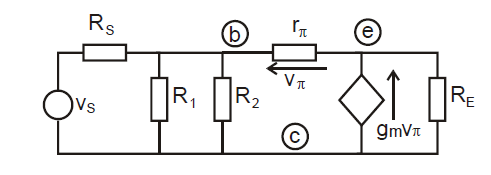
\includegraphics[width=10cm]{figures/ss_collector}}
	\caption{Common emitter stage}
	\label{fig:ss_collector}
	\hfill
\end{figure}

By using KVL on the emitter terminal we can establish that 
\begin{align}
\frac{v_e - v_s}{r_\pi} + g_m v_\pi +\frac{v_e}{R_E} &= 0 \label{eq:emitter2} \\
\frac{v_e - v_s}{r_\pi} + g_m (v_e - v_s) +\frac{v_e}{R_E} &= 0 \nonumber \\
\frac{v_e - v_s}{r_\pi} + \frac{\beta (v_e - v_s)}{r_\pi} +\frac{v_e}{R_E} &= 0 \nonumber \\
v_e(\beta R_E + R_E + r_\pi) &= v_s R_E(\beta + 1) \nonumber \\
\frac{v_e}{v_s} &= \frac{R_E (\beta + 1)}{R_E (\beta + 1) + r_\pi} \label{eq:collector_gain}
\end{align}

Therefore gain $\approx 1$

\subsection{Input Impedance}
Input impedance 
\begin{align}
R_i &= \frac{v_s}{i_b} \label{eq:Ri}
\end{align}

Neglecting $R_1, R_2$ and $R_s$ gives

\begin{align*}
i_b &= \frac{v_s-v_e}{r_\pi} 
\end{align*}

Substituting equation \ref{eq:collector_gain} into this gives
\begin{align}
i_b &= \frac{v_s}{r_\pi} - \frac{v_s}{r_\pi} (\frac{R_E (\beta + 1)}{R_E (\beta + 1) + r_\pi}) \nonumber \\
&= \frac{v_s}{r_\pi} (1- \frac{R_E (\beta + 1)}{R_E (\beta + 1) + r_\pi}) \nonumber \\
&= \frac{v_s}{R_E (\beta + 1) + r_\pi} \label{eq:ib}
\end{align}

Therefore combining \ref{eq:Ri} and \ref{eq:ib} gives 
\begin{align}
R_i = \frac{v_s}{i_b} = R_E (\beta + 1) + r_\pi \label{eq:collector_input_imp}
\end{align}

\subsubsection{Output Impedance}
\begin{figure}[H]
	\centering
	\subfloat{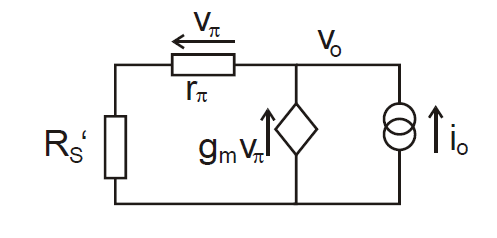
\includegraphics[width=10cm]{figures/o_imp_collector}}
	\caption{Common emitter stage}
	\label{fig:o_imp_collector}
	\hfill
\end{figure}

In figure \ref{fig:o_imp_collector} the Thevenin equivalent of the source resistances has been taken ($R_s'$)
\begin{align*}
R_s' = R_s || R_1 || R_2
\end{align*}

By KVL 
\begin{align}
i_o + g_m v_\pi - \frac{v_o}{r_\pi R_s'} &= 0 \label{eq:KVL}\\
v_\pi &= - \frac{r_\pi v_o}{r_\pi + R_s'} \label{eq:vpi}
\end{align}

Substituting equation \ref{eq:KVL} into \ref{eq:vpi} gives
\begin{align}
i_o -g_m \frac{r_\pi v_o}{r_\pi + R_s'} - \frac{v_o}{r_\pi R_s'} &= 0 \nonumber \\
\frac{v_o (1 + g_m r_\pi)}{r_\pi + R_s'} &= i_b \nonumber \\
R_o = \frac{v_o}{i_b} &= \frac{r_\pi + R_s'}{1 + \beta} \label{eq:output_imp_collector}
\end{align}


\section{Simulation}

Used MATLAB program to calculate values for each of the resistors and capacitors. 

\begin{figure}[H]
	\centering
	% Requires \usepackage{graphicx}
	\subfloat[Schematic for common collector amplifier]{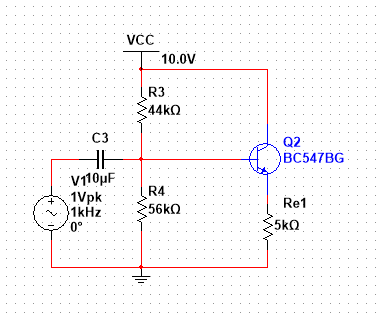
\includegraphics[width=7cm]{figures/sch_col}\label{add}}
	\hspace{0.5cm}
	\subfloat[Schematic for common emitter amplifier]{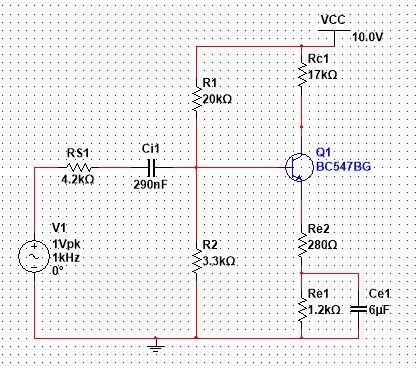
\includegraphics[width=7cm]{figures/sch_em}\label{sub}}	
\end{figure}


\begin{figure}[H]
	\centering
	\subfloat{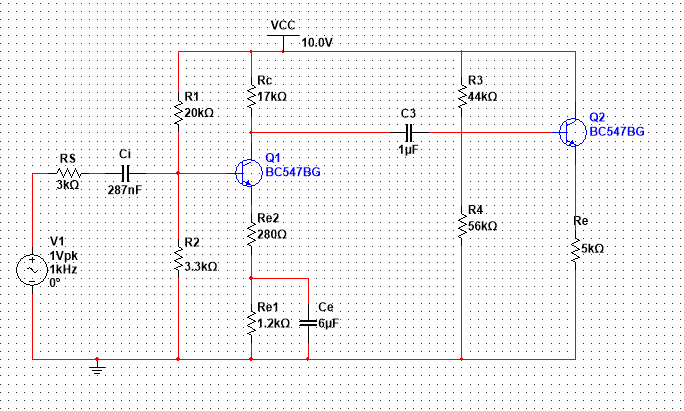
\includegraphics[width=18cm]{figures/sch_full}}
	\caption{Schematic for full amplifier featuring both stages connected}
	\label{fig:sch_full}
	\hfill
\end{figure}

\begin{figure}[H]
	\centering
	\subfloat{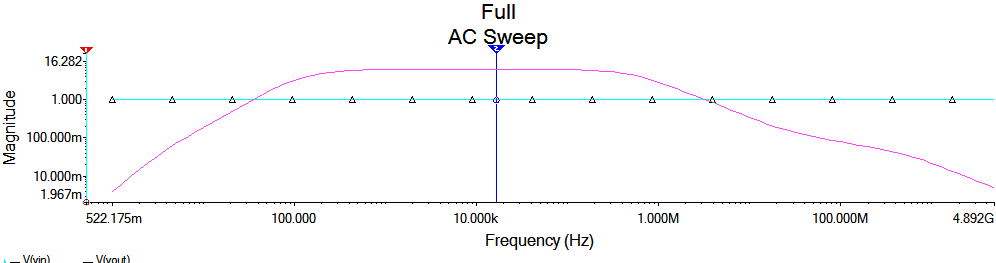
\includegraphics[width=18cm]{figures/sim_full}}
	\caption{Simulation for the combined amplifier}
	\label{fig:sim_full}
	\hfill
\end{figure}

\begin{figure}[H]
	\centering
	\subfloat{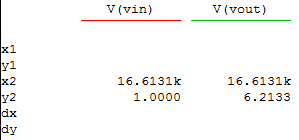
\includegraphics[width=8cm]{figures/sim_full_cursors}}
	\label{fig:sim_full_cursors}
	\hfill
\end{figure}

Gain of 6.2133 from the simulation. \\
Input impedance \num{3.1150e+05}\\
Output impedance 143.2382\\

\vspace{10mm}
Output impedance stage 1 \num{17e3}\\
Input impedance stage 2 \num{1e6}\\

Therefore $10 R_{o1} \ll R_{i2} $

%\nocite{*}
%\bibliographystyle{IEEETran}
%\bibliography{Report}

\begin{appendices}

\end{appendices}


\end{document}